% luatikztutorial.tex
\documentclass[lualatex]{jlreq}
% 00preamble.tex
% 基本とドライバ関連
\usepackage{graphicx}
\usepackage[table]{xcolor}
\usepackage{geometry}
\usepackage{siunitx}
\usepackage{multirow}
\usepackage{float}
\usepackage{url}
\usepackage{listings}
\usepackage{caption2}
\usepackage{lscape}
\usepackage{pdflscape}
\usepackage{csvsimple}
\usepackage{wrapfig}
\usepackage{comment}
\usepackage{cprotect}
\usepackage{tikz}
\usetikzlibrary{intersections, calc, arrows.meta}
\usetikzlibrary{positioning, through}
\usepackage{fancybox}
\usepackage{booktabs}
\usepackage{adjustbox}
\usepackage{longtable}
\usepackage{nameref}
% 数式系パッケージ
\usepackage{amsmath,amssymb,amsfonts}
\usepackage{mathtools,amssymb,amsfonts}
\usepackage{amsthm}
\usepackage{bm}
% LuaTeX-ja設定
\usepackage{luatexja}
\usepackage[no-math]{luatexja-fontspec}

\setcounter{section}{0}
\makeatletter
    \renewcommand{\theequation}{
    \thesection.\arabic{equation}}
    \@addtoreset{equation}{section}
    \renewcommand{\figurename}{Figure }
    \renewcommand{\tablename}{Table }
\makeatother
\geometry{top=15truemm,bottom=25.4truemm,inner=19.05truemm,outer=19.05truemm}

% Remove section number from equation number, so that it is just 1, 2, NOT 1.1, 2.1:
% \counterwithout{equation}{section}

% Source code listing settings (listings package)
\lstset{
    frame=tb,
    basicstyle=\ttfamily\small,
    % basicstyle=\ttfamily\small\bfseries,
    columns=fullflexible,
    keepspaces=true,
    numbers=left,
    firstnumber=1,
    numberstyle=\scriptsize,
    breaklines=true,
    % frame=none
    % frame=single,
    % gobble=4,
    % xleftmargin=0.2\textwidth,
    % xrightmargin=0.2\textwidth,
}
% \renewcommand{\lstlistlistingname}{List of Source Codes}
% \renewcommand{\lstlistingname}{リスト}

\NewDocumentCommand{\bissectrice}{%
    O{}     % drawing options
    mmm     % bissector of mmm
    m       % intersection point between base and bissector
    O{1}O{1}% extended drawing of the bissector
    }{%
    \path[name path=Bis#2#3#4] let
        \p1 = ($(#2) - (#3)$),          % chktex 46
        \p2 = ($(#4) - (#3)$),          % chktex 46
        \n1 = {veclen(\x1,\y1)},        % chktex 36
        \n2 = {veclen(\x2,\y2)},        % chktex 36
        \n3 = {max(\n1,\n2)},           % chktex 36
        \p1 = ($(#3)!\n3!(#2)$),        % chktex 46
        \p2 = ($(#3)!\n3!(#4)$),        % chktex 46
        \p3 = ($(\p1) + (\p2) - (#3)$)  % chktex 46
    in
        (#3) --(\p3);                   % chktex 36

    \path[name path = foo] (#2) --(#4); % chktex 36

    \path[name intersections={of=foo and Bis#2#3#4, by=#5}];

    \path[#1] ($(#3)!#6!(#5)$) --($(#5)!#7!(#3)$); % chktex 46, chktex 36
}


\counterwithout{equation}{section}
\geometry{top=20truemm,bottom=25.4truemm,inner=19.05truemm,outer=19.05truemm}
\title{\bfseries {\huge Test of 「\LaTeX{}で図を直接描けるTikZの使い方」}}
\author{\LARGE Ivan Setiawan}
\author{{\LARGE Ivan Setiawan\thanks{MyCompany, Inc.}} \and {\LARGE My Self\,\thanks{株式会社マイカンパニー}}}
\date{Created: 2026年4月17日\\[0.3em]Last Updated: 2026/04/28}

\renewcommand{\lstlistlistingname}{\LaTeX{} TikZ codelistの一覧}
\renewcommand{\lstlistingname}{リスト}
\renewcommand{\tablename}{表}
\renewcommand{\listtablename}{表の一覧}

\begin{document}
\maketitle
\hrule

\lstlistoflistings{}
\vspace{0.5em}
\hrule

\listoftables
\vspace{0.5em}
\hrule

\vspace{1em}

\section*{Always use TikZ inside \texttt{tikzpicture} environment}

TikZ command can be used in its shortened form like below:
\vspace{0.5em}
\begin{center}
    \begin{Sbox}
        \begin{minipage}{0.8 \textwidth}
            \begin{verbatim*}
                \tikz{\draw 〜〜〜〜}
                \tikz \draw 〜〜〜〜;\end{verbatim*}
        \end{minipage}
    \end{Sbox}
    \shadowbox{\TheSbox}
\end{center}
However, the \texttt{chktex} program will give a lot of warnings if TikZ is used in this shortened form. Therefore, it is recommended to use TikZ commands inside the \texttt{tikzpicture} environment.

\section*{Inline mode \texttt{tikzpicture} environment}

Both syntaxes below are valid for using TikZ in inline mode:
\vspace{0.5em}
\begin{center}
    \begin{Sbox}
        \begin{minipage}{0.8 \textwidth}
            \begin{verbatim}
\begin{tikzpicture}
    \draw 〜〜〜〜;
\end{tikzpicture}

\(
\begin{tikzpicture}
    \draw 〜〜〜〜;
\end{tikzpicture}
\) \end{verbatim}
        \end{minipage}
    \end{Sbox}
    \shadowbox{\TheSbox}
\end{center}

So, when we write like this:
\vspace{0.5em}
\begin{center}
    \begin{Sbox}
        \begin{minipage}{0.8 \textwidth}
            \begin{verbatim}
``An example of inline TikZ:\
\begin{tikzpicture}
    \draw (0,0) -- (2,1);
\end{tikzpicture}
inside a sentence''\end{verbatim}
        \end{minipage}
    \end{Sbox}
    \fbox{\TheSbox}
\end{center}
, we get
``An example of inline TikZ:\
\begin{tikzpicture}
    \draw (0,0) -- (2,1);
\end{tikzpicture}
inside a sentence''.

Also, when we write like this:
\vspace{0.5em}
\begin{center}
    \begin{Sbox}
        \begin{minipage}{0.8 \textwidth}
            \begin{verbatim}
``Now, an example of inline math and TikZ:\
\(
\alpha + \beta = \gamma \,
\begin{tikzpicture}
    \draw (0,0) -- (2,1);
\end{tikzpicture}
\)
inside a sentence''\end{verbatim}
        \end{minipage}
    \end{Sbox}
    \fbox{\TheSbox}
\end{center}
, we get
``Now, an example of inline math and TikZ:\
\(
\alpha + \beta = \gamma \,
\begin{tikzpicture}
    \draw (0,0) -- (2,1);
\end{tikzpicture}
\)
inside a sentence''.

\section*{Display mode \texttt{tikzpicture} environment}

Use below syntax for using TikZ in display mode:
\vspace{0.5em}
\begin{center}
    \begin{Sbox}
        \begin{minipage}{0.8 \textwidth}
            \begin{verbatim}
\[
\begin{tikzpicture}
    \draw 〜〜〜〜;
\end{tikzpicture}
\] \end{verbatim}
        \end{minipage}
    \end{Sbox}
    \shadowbox{\TheSbox}
\end{center}

So, when we write like this:
\begin{lstlisting}[language={[LaTeX] TeX},frame=single,xleftmargin=0.2 \textwidth,xrightmargin=0.2 \textwidth,breaklines=true,]
``Finally, an example of display math and TikZ:\
\[
    \alpha^2 + \beta^2 = \gamma^2 \,
    \begin{tikzpicture}
        \draw (0,0) -- (2,-1);
    \end{tikzpicture}
\]
''
\end{lstlisting}
, we get
``Finally, an example of display math and TikZ:\
\[
    \alpha^2 + \beta^2 = \gamma^2 \,
    \begin{tikzpicture}
        \draw (0,0) -- (2,-1);
    \end{tikzpicture}
\]
''.

\section*{Good TikZ manual}

「TikZ の使い方」, which is available in \url{https://alg-d.com/math/tikz.pdf}.

The massive document for TikZ can be opened with the command line \texttt{texdoc tikz}.

\section{「\LaTeX{}で図を直接描けるTikZの使い方１｜基本的な描線」}
\label{linebasic}

第~\ref{linebasic}章では，\url{https://math-note.xyz/latex/tikz/tikz-line/}にあるコードを，いくつか試してみる．

リスト~\ref{lst:straightline}で，線を描く．略記方では，\verb*|\tikz| の後ろに，命令を書いて，最後に ``;'' (semicolon)で命令を閉じなければならない．しかし，略記方の場合は，\texttt{chktex}の false positive (warning)が多いので，\texttt{tikzpicture}環境で使うことが推奨される．
\begin{lstlisting}[language={[LaTeX] TeX},caption={直線を描く},label={lst:straightline},firstnumber=1,breaklines=true,gobble=4,]
    \begin{tikzpicture}
        \draw (0,0) -- (2,0);
    \end{tikzpicture}
\end{lstlisting}
上記のコマンドは，次のような「本文中の」直線：
\begin{tikzpicture}
    \draw (0,0) -- (2,0);
\end{tikzpicture}
，になる．

表~\ref{tab:basictikzcommandoutput}に TikZ コマンドと対応する出力を示す．\LaTeX{} コマンドは，\verb|\begin{tikzpicture}| と \verb|\end{tikzpicture}| との間に囲んで，使うこと．

\newcommand{\cwA}{5.5cm} % column 1's width (macro cannot have number as identifier)
\newcommand{\cwB}{4cm} % column 2's width
\newcommand{\cwC}{5.5cm} % column 3's width
\newcommand{\tablerowseparatorline}{
    \addlinespace[0.3em]
    \cmidrule{1-3}
    \addlinespace[0.2em]
}
\begin{longtable}{p{\cwA} p{\cwB} p{\cwC}}
    \caption{基礎TikZコマンドとその出力} \label{tab:basictikzcommandoutput}                                      \\[-1em]
    \toprule
    \textbf{Command} & \textbf{Rendered Output} & \textbf{説明}                                         \\
    \midrule
    \endfirsthead % chktex 1

    % \midrule
    \multicolumn{3}{c}{表~\ref{tab:basictikzcommandoutput}:~\nameref{tab:basictikzcommandoutput}（の続き）} \\[0.3em]
    \toprule
    \textbf{Command} & \textbf{Rendered Output} & \textbf{説明}                                         \\
    \midrule
    \endhead % chktex 1

    % \midrule
    \multicolumn{3}{r}{表~\ref{tab:basictikzcommandoutput}（次のページへ続く）}                                  \\
    \midrule
    \endfoot % chktex 1

    \midrule
    \multicolumn{3}{r}{表~\ref{tab:basictikzcommandoutput}終了}                                          \\
    \bottomrule
    \endlastfoot % chktex 1

    \begin{adjustbox}{valign=t,minipage=\cwA}
        \begin{lstlisting}[language={[LaTeX] TeX},numbers=none,frame=none,breaklines=true,aboveskip=0em,belowskip=0em,gobble=12,]
            \draw (0,0)--(2,1.5);
        \end{lstlisting}
    \end{adjustbox}
                     &
    \begin{adjustbox}{valign=t,minipage=\cwB}
        \begin{tikzpicture}
            \draw (0,0)--(2,1.5);
        \end{tikzpicture}
    \end{adjustbox}
                     &
    \begin{adjustbox}{valign=t,minipage=\cwC}
        (0,0) から (\qty{2}{\cm}, \qty{1.5}{\cm}) まで線分を引く
    \end{adjustbox}
    \\
    \tablerowseparatorline{}
    \begin{adjustbox}{valign=t,minipage=\cwA}
        \begin{lstlisting}[language={[LaTeX] TeX},numbers=none,frame=none,breaklines=true,aboveskip=0em,belowskip=0em,gobble=12,]
            \draw (0+7,0+8)--(2+7,1.5+8);
        \end{lstlisting}
    \end{adjustbox}
                     &
    \begin{adjustbox}{valign=t,minipage=\cwB}
        \begin{tikzpicture}
            \draw (0+7,0+8)--(2+7,1.5+8);
        \end{tikzpicture}
    \end{adjustbox}
                     &
    \begin{adjustbox}{valign=t,minipage=\cwC}
        並行移動しても表示されたりせず，上と同じく
    \end{adjustbox}
    \\
    \tablerowseparatorline{}
    \begin{adjustbox}{valign=t,minipage=\cwA}
        \begin{lstlisting}[language={[LaTeX] TeX},numbers=none,frame=none,breaklines=true,aboveskip=0em,belowskip=0em,gobble=12,]
            \draw (0,0)--(2,0);
            \draw (1,1)--(3,1);
            \draw (-1,-1)--(2,-1.5) (2,-1)--(-1,-1.5);
        \end{lstlisting}
    \end{adjustbox}
                     &
    \begin{adjustbox}{valign=t,minipage=\cwB}
        \begin{tikzpicture}
            \draw (0,0)--(2,0);
            \draw (1,1)--(3,1);
            \draw (-0.5,-1)--(2,-1.5) (2,-1)--(-0.5,-1.5);
        \end{tikzpicture}
    \end{adjustbox}
                     &
    \begin{adjustbox}{valign=t,minipage=\cwC}
        1本ごとに \verb|\draw| を書くか，1つの \verb|\draw| の後ろに複数本を書く
    \end{adjustbox}
    \\
    \tablerowseparatorline{}
    \begin{adjustbox}{valign=t,minipage=\cwA}
        \begin{lstlisting}[language={[LaTeX] TeX},numbers=none,frame=none,breaklines=true,aboveskip=0em,belowskip=0em,gobble=12,]
            \draw[ultra thick] (0,0)--(2,1)--(3,-1)--cycle;
        \end{lstlisting}
    \end{adjustbox}
                     &
    \begin{adjustbox}{valign=t,minipage=\cwB}
        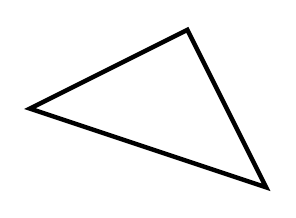
\begin{tikzpicture}
            \draw[ultra thick] (0,0)--(2,1)--(3,-1)--cycle;
        \end{tikzpicture}
    \end{adjustbox}
                     &
    \begin{adjustbox}{valign=t,minipage=\cwC}
        線を閉じるときは，\verb|--cycle| を使う．太い線を描く時に，\verb|--cycle| だとキレイに閉じる
    \end{adjustbox}
    \\
    \tablerowseparatorline{}
    \begin{adjustbox}{valign=t,minipage=\cwA}
        \begin{lstlisting}[language={[LaTeX] TeX},numbers=none,frame=none,breaklines=true,aboveskip=0em,belowskip=0em,gobble=12,]
            \draw (0,0) rectangle (3,2);
        \end{lstlisting}
    \end{adjustbox}
                     &
    \begin{adjustbox}{valign=t,minipage=\cwB}
        \begin{tikzpicture}
            \draw (0,0) rectangle (3,2);
        \end{tikzpicture}
    \end{adjustbox}
                     &
    \begin{adjustbox}{valign=t,minipage=\cwC}
        (0,0) から (3,2) への対角線を持った四角形を描く
    \end{adjustbox}
    \\
    \tablerowseparatorline{}
    \begin{adjustbox}{valign=t,minipage=\cwA}
        \begin{lstlisting}[language={[LaTeX] TeX},numbers=none,frame=none,breaklines=true,aboveskip=0em,belowskip=0em,gobble=12,]
            \draw (0,0) -- (3,0);
            \draw (1,1) -- ($(0,0)!(1,1)!(3,0)$);
        \end{lstlisting}
    \end{adjustbox}
                     &
    \begin{adjustbox}{valign=t,minipage=\cwB}
        \begin{tikzpicture}
            \draw (0,0) -- (3,0);
            \draw (1,1) -- ($(0,0)!(1,1)!(3,0)$);
        \end{tikzpicture}
    \end{adjustbox}
                     &
    \begin{adjustbox}{valign=t,minipage=\cwC}
        \verb|($(0,0)!(1,1)!(3,0)$)| は，線分 \verb|(0,0) -- (3,0)| に点 (1,1) から下ろした「垂線の足」である
    \end{adjustbox}
    \\
    \addlinespace[0.3em]
\end{longtable}

表~\ref{tab:circle}は円や楕円のTikZコマンドをまとめる．
\begin{table}[h]
    \centering
    \caption{円や楕円のTikZコマンドとその出力} \label{tab:circle}
    \vspace{0.5em}
    \begin{tabular}{p{\cwA} p{\cwB} p{\cwC}}
        \toprule
        \textbf{Command} & \textbf{Rendered Output} & \textbf{説明} \\
        \midrule
        \begin{adjustbox}{valign=t,minipage=\cwA}
            \begin{lstlisting}[language={[LaTeX] TeX},numbers=none,frame=none,breaklines=true,aboveskip=0em,belowskip=0em,gobble=16,]
                \draw (0,0) circle[radius=1];
                \draw (1,1) circle[radius=2];
            \end{lstlisting}
        \end{adjustbox}
                         &
        \begin{adjustbox}{valign=t,minipage=\cwB}
            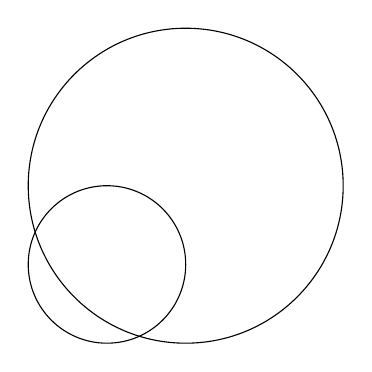
\begin{tikzpicture}
                \draw (0,0) circle[radius=1];
                \draw (1,1) circle[radius=2];
            \end{tikzpicture}
        \end{adjustbox}
                         &
        \begin{adjustbox}{valign=t,minipage=\cwC}
            (0,0)を中心に半径 \qty{1}{\cm}と， (1,1)を中心に半径 \qty{2}{\cm}の2つの円
        \end{adjustbox}
        \\
        \tablerowseparatorline{}
        \begin{adjustbox}{valign=t,minipage=\cwA}
            \begin{lstlisting}[language={[LaTeX] TeX},numbers=none,frame=none,breaklines=true,aboveskip=0em,belowskip=0em,gobble=16,]
                \draw(0,0) circle [x radius=1.5, y radius=0.5, rotate=30];
            \end{lstlisting}
        \end{adjustbox}
                         &
        \begin{adjustbox}{valign=t,minipage=\cwB}
            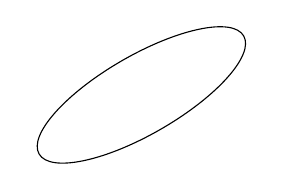
\begin{tikzpicture}
                \draw(0,0) circle [x radius=1.5, y radius=0.5, rotate=30];
            \end{tikzpicture}
        \end{adjustbox}
                         &
        \begin{adjustbox}{valign=t,minipage=\cwC}
            点~(0,0)中心，第1成分の径の長さが \qty{1.5}{\cm}，第2成分の径の長さが \qty{0.5}{\cm}の楕円を30°傾けた
        \end{adjustbox}
        \\
        \addlinespace[0.3em]
        \bottomrule
    \end{tabular}
\end{table}

表~\ref{tab:arcrotate}は円弧 (arc) と \texttt{rotate} と文字 \texttt{node} についてまとめる．
\begin{longtable}{p{\cwA} p{\cwB} p{\cwC}}
    \caption{円弧 (arc) と \texttt{rotate} と文字 \texttt{node}} \label{tab:arcrotate} \\[-1em]
    \toprule
    \textbf{Command} & \textbf{Rendered Output} & \textbf{説明}                    \\
    \midrule
    \endfirsthead % chktex 1

    % \midrule
    \multicolumn{3}{c}{表~\ref{tab:arcrotate}:~\nameref{tab:arcrotate}（の続き）}      \\[0.3em]
    \toprule
    \textbf{Command} & \textbf{Rendered Output} & \textbf{説明}                    \\
    \midrule
    \endhead % chktex 1

    % \midrule
    \multicolumn{3}{r}{表~\ref{tab:arcrotate}（次のページへ続く）}                          \\
    \midrule
    \endfoot % chktex 1

    \midrule
    \multicolumn{3}{r}{表~\ref{tab:arcrotate}終了}                                  \\
    \bottomrule
    \endlastfoot % chktex 1

    \begin{adjustbox}{valign=t,minipage=\cwA}
        \begin{lstlisting}[language={[LaTeX] TeX},numbers=none,frame=none,breaklines=true,aboveskip=0em,belowskip=0em,gobble=12,]
            \draw (0,0) arc (30:70:3);
        \end{lstlisting}
    \end{adjustbox}
                     &
    \begin{adjustbox}{valign=t,minipage=\cwB}
        \begin{tikzpicture}
            \draw (0,0) arc (30:70:3);
        \end{tikzpicture}
    \end{adjustbox}
                     &
    \begin{adjustbox}{valign=t,minipage=\cwC}
        (0,0) から始まる半径 \qty{3}{\cm} の円の偏角 \qty{30}{\degree} から \qty{70}{\degree} までの弧
    \end{adjustbox}
    \\
    \tablerowseparatorline{}
    \begin{adjustbox}{valign=t,minipage=\cwA}
        \begin{lstlisting}[language={[LaTeX] TeX},numbers=none,frame=none,breaklines=true,aboveskip=0em,belowskip=0em,gobble=12,]
            \draw (0,0) arc [start angle=0, end angle=90, x radius = 2, y radius=1];
        \end{lstlisting}
    \end{adjustbox}
                     &
    \begin{adjustbox}{valign=t,minipage=\cwB}
        \begin{tikzpicture}
            \draw (0,0) arc [start angle=0, end angle=90, x radius = 2, y radius=1];
        \end{tikzpicture}
    \end{adjustbox}
                     &
    \begin{adjustbox}{valign=t,minipage=\cwC}
        (0,0) から始まる第1成分の径が \qty{2}{\cm} と第2成分の径が \qty{1}{\cm} の楕円の偏角 \qty{0}{\degree} から \qty{90}{\degree} までの弧
    \end{adjustbox}
    \\
    \tablerowseparatorline{}
    \begin{adjustbox}{valign=t,minipage=\cwA}
        \begin{lstlisting}[language={[LaTeX] TeX},numbers=none,frame=none,breaklines=true,aboveskip=0em,belowskip=0em,gobble=12,]
            \draw (0,0) to [out=45, in=135] (4,0);
        \end{lstlisting}
    \end{adjustbox}
                     &
    \begin{adjustbox}{valign=t,minipage=\cwB}
        \begin{tikzpicture}
            \draw (0,0) to [out=45, in=135] (4,0);
        \end{tikzpicture}
    \end{adjustbox}
                     &
    \begin{adjustbox}{valign=t,minipage=\cwC}
        (0,0) から偏角 \qty{45}{\degree} の方向へ出て， (4,0) へ偏角 \qty{135}{\degree} の方向から入る曲線
    \end{adjustbox}
    \\
    \tablerowseparatorline{}
    \begin{adjustbox}{valign=t,minipage=\cwA}
        \begin{lstlisting}[language={[LaTeX] TeX},numbers=none,frame=none,breaklines=true,aboveskip=0em,belowskip=0em,gobble=12,]
            \draw (0,0) to [out=45, in=135, relative] ({sqrt(2)},{sqrt(2)});
        \end{lstlisting}
    \end{adjustbox}
                     &
    \begin{adjustbox}{valign=t,minipage=\cwB}
        \begin{tikzpicture}
            \draw (0,0) to [out=45, in=135, relative] ({sqrt(2)},{sqrt(2)});
        \end{tikzpicture}
    \end{adjustbox}
                     &
    \begin{adjustbox}{valign=t,minipage=\cwC}
        ``relative'' を記述することで，2点を結ぶ線分は偏角の基準軸となる
    \end{adjustbox}
    \\
    \tablerowseparatorline{}
    \begin{adjustbox}{valign=t,minipage=\cwA}
        \begin{lstlisting}[language={[LaTeX] TeX},numbers=none,frame=none,breaklines=true,aboveskip=0em,belowskip=0em,gobble=12,]
            \draw[rotate=45] (0,0) to [out=45, in=135] (3,0);
        \end{lstlisting}
    \end{adjustbox}
                     &
    \begin{adjustbox}{valign=t,minipage=\cwB}
        \begin{tikzpicture}
            \draw[rotate=45] (0,0) to [out=45, in=135] (3,0);
        \end{tikzpicture}
    \end{adjustbox}
                     &
    \begin{adjustbox}{valign=t,minipage=\cwC}
        回転するだけなら，\verb|\draw| の直後に \verb|[rotate=角度]| というオプションを使えば良い
    \end{adjustbox}
    \\
    \tablerowseparatorline{}
    \begin{adjustbox}{valign=t,minipage=\cwA}
        \begin{lstlisting}[language={[LaTeX] TeX},numbers=none,frame=none,breaklines=true,aboveskip=0em,belowskip=0em,gobble=12,]
            \draw (0,0) to [out=45, in=135] (3,3);
        \end{lstlisting}
    \end{adjustbox}
                     &
    \begin{adjustbox}{valign=t,minipage=\cwB}
        \begin{tikzpicture}
            \draw (0,0) to [out=45,in=135] (3,3);
        \end{tikzpicture}
    \end{adjustbox}
                     &
    \begin{adjustbox}{valign=t,minipage=\cwC}
        偏角の基準軸は \(x \) 軸正方向からの偏角であることに注意
    \end{adjustbox}
    \\
    \tablerowseparatorline{}
    \begin{adjustbox}{valign=t,minipage=\cwA}
        \begin{lstlisting}[language={[LaTeX] TeX},numbers=none,frame=none,breaklines=true,aboveskip=0em,belowskip=0em,gobble=12,]
            \draw (0,0) -- (2,1) -- (3,-1) -- (1,-1) -- cycle;
            \draw (0,0) node{A};
            \draw (2,1) node{B};
            \draw (3,-1) node{C};
            \draw (1,-1) node{D};
        \end{lstlisting}
    \end{adjustbox}
                     &
    \begin{adjustbox}{valign=t,minipage=\cwB}
        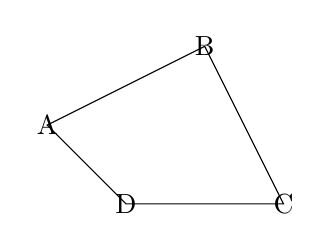
\begin{tikzpicture}
            \draw (0,0) -- (2,1) -- (3,-1) -- (1,-1) -- cycle;
            \draw (0,0) node{A};
            \draw (2,1) node{B};
            \draw (3,-1) node{C};
            \draw (1,-1) node{D};
        \end{tikzpicture}
    \end{adjustbox}
                     &
    \begin{adjustbox}{valign=t,minipage=\cwC}
        \texttt{node} で文字を書き込む
    \end{adjustbox}
    \\
    \tablerowseparatorline{}
    \begin{adjustbox}{valign=t,minipage=\cwA}
        \begin{lstlisting}[language={[LaTeX] TeX},numbers=none,frame=none,breaklines=true,aboveskip=0em,belowskip=0em,gobble=12,]
            \draw (0,0) -- (2,1) -- (3,-1) -- (1,-1) -- cycle;
            \draw (0,0) node[left]{A};
            \draw (2,1) node[above]{B};
            \draw (3,-1) node[right]{C};
            \draw (1,-1) node[below left]{D};
        \end{lstlisting}
    \end{adjustbox}
                     &
    \begin{adjustbox}{valign=t,minipage=\cwB}
        \begin{tikzpicture}
            \draw (0,0) -- (2,1) -- (3,-1) -- (1,-1) -- cycle;
            \draw (0,0) node[left]{A};
            \draw (2,1) node[above]{B};
            \draw (3,-1) node[right]{C};
            \draw (1,-1) node[below left]{D};
        \end{tikzpicture}
    \end{adjustbox}
                     &
    \begin{adjustbox}{valign=t,minipage=\cwC}
        \texttt{node} でオプションを使えば文字を動かせる
    \end{adjustbox}
    \\
    \tablerowseparatorline{}
    \begin{adjustbox}{valign=t,minipage=\cwA}
        \begin{lstlisting}[language={[LaTeX] TeX},numbers=none,frame=none,breaklines=true,aboveskip=0em,belowskip=0em,gobble=12,]
            \draw (0,0) node[left]{A} -- (2,1) node[above]{B} -- (3,-1) node[right]{C} -- (1,-1) node[below left]{D}
            - cycle;
\end{lstlisting}
    \end{adjustbox}
                     &
    \begin{adjustbox}{valign=t,minipage=\cwB}
        \begin{tikzpicture}
            \draw (0,0) node[left]{A} -- (2,1) node[above]{B} -- (3,-1) node[right]{C} -- (1,-1) node[below left]{D} -- cycle;
        \end{tikzpicture}
    \end{adjustbox}
                     &
    \begin{adjustbox}{valign=t,minipage=\cwC}
        \texttt{node} can also be written inside the broken line \verb|\draw|
    \end{adjustbox}
    \\
    \addlinespace[0.3em]
\end{longtable}

\section{「\LaTeX{}で図を直接描けるTikZの使い方２｜線のスタイル」}
\label{linestyle}

第~\ref{linestyle}章では，\url{https://math-note.xyz/latex/tikz/tikz-style/}にあるコードを，いくつか試してみる．

表~\ref{tab:linestylecolor}は線分や arc のスタイルや色についてまとめる．
\begin{longtable}{p{\cwA} p{\cwB} p{\cwC}}
    \caption{線分や arc のスタイルや色を制御するTikZコマンド} \label{tab:linestylecolor}                 \\[-1em]
    \toprule
    \textbf{Command} & \textbf{Rendered Output} & \textbf{説明}                         \\
    \midrule
    \endfirsthead % chktex 1

    % \midrule
    \multicolumn{3}{c}{表~\ref{tab:linestylecolor}:~\nameref{tab:linestylecolor}（の続き）} \\[0.3em]
    \toprule
    \textbf{Command} & \textbf{Rendered Output} & \textbf{説明}                         \\
    \midrule
    \endhead % chktex 1

    % \midrule
    \multicolumn{3}{r}{表~\ref{tab:linestylecolor}（次のページへ続く）}                          \\
    \midrule
    \endfoot % chktex 1

    \midrule
    \multicolumn{3}{r}{表~\ref{tab:linestylecolor}終了}                                  \\
    \bottomrule
    \endlastfoot % chktex 1

    \begin{adjustbox}{valign=t,minipage=\cwA}
        \begin{lstlisting}[language={[LaTeX] TeX},numbers=none,frame=none,breaklines=true,aboveskip=0em,belowskip=0em,gobble=12,]
            \draw[line width=1pt] (0,0) -- (2,0);
        \end{lstlisting}
    \end{adjustbox}
                     &
    \begin{adjustbox}{valign=t,minipage=\cwB}
        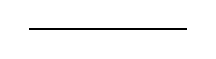
\begin{tikzpicture}
            \draw[line width=1pt] (0,0) -- (2,0);
        \end{tikzpicture}
    \end{adjustbox}
                     &
    \begin{adjustbox}{valign=t,minipage=\cwC}
        太さ \qty{1}{pt} の線分
    \end{adjustbox}
    \\
    \tablerowseparatorline{}
    \begin{adjustbox}{valign=t,minipage=\cwA}
        \begin{lstlisting}[language={[LaTeX] TeX},numbers=none,frame=none,breaklines=true,aboveskip=0em,belowskip=0em,gobble=12,]
            \draw[ultra thin] (0,0) -- (2,0);
            \draw[thin] (0,-0.5) -- (2,-0.5);
            \draw[semithick] (0,-1.0) -- (2,-1.0);
            \draw[thick] (0,-1.5) -- (2,-1.5);
            \draw[ultra thick] (0,-2.0) -- (2,-2.0);
        \end{lstlisting}
    \end{adjustbox}
                     &
    \begin{adjustbox}{valign=t,minipage=\cwB}
        
\begin{tikzpicture}
            \draw[ultra thin] (0,0) -- (2,0);
            \draw[thin] (0,-0.5) -- (2,-0.5);
            \draw[semithick] (0,-1.0) -- (2,-1.0);
            \draw[thick] (0,-1.5) -- (2,-1.5);
            \draw[ultra thick] (0,-2.0) -- (2,-2.0);
        \end{tikzpicture}
    \end{adjustbox}
                     &
    \begin{adjustbox}{valign=t,minipage=\cwC}
        \texttt{ultra thin, very thin, thin, semithick, thick, very thick, ultra thick}
    \end{adjustbox}
    \\
    \tablerowseparatorline{}
    \begin{adjustbox}{valign=t,minipage=\cwA}
        \begin{lstlisting}[language={[LaTeX] TeX},numbers=none,frame=none,breaklines=true,aboveskip=0em,belowskip=0em,gobble=12,]
            \draw[dash pattern=on 3pt off 2pt on 5pt off 2pt] (0,0) -- (4,0);
        \end{lstlisting}
    \end{adjustbox}
                     &
    \begin{adjustbox}{valign=t,minipage=\cwB}
        \begin{tikzpicture}
            \draw[dash pattern=on 3pt off 2pt on 5pt off 2pt] (0,0) -- (4,0);
        \end{tikzpicture}
    \end{adjustbox}
                     &
    \begin{adjustbox}{valign=t,minipage=\cwC}
        オプション \verb|dash pattern| に \verb|on off| を指定して，点破線のデザインができる
    \end{adjustbox}
    \\
    \tablerowseparatorline{}
    \begin{adjustbox}{valign=t,minipage=\cwA}
        \begin{lstlisting}[language={[LaTeX] TeX},numbers=none,frame=none,breaklines=true,aboveskip=0em,belowskip=0em,gobble=12,]
            \draw[dotted] (0,0) -- (2,0);
            \draw[dashed] (0,-0.5) -- (2,-0.5);
            \draw[dash dot] (0,-1.0) -- (2,-1.0);
            \draw[dash dot dot] (0,-1.5) -- (2,-1.5);
        \end{lstlisting}
    \end{adjustbox}
                     &
    \begin{adjustbox}{valign=t,minipage=\cwB}
        \begin{tikzpicture}
            \draw[dotted] (0,0) -- (2,0);
            \draw[dashed] (0,-0.5) -- (2,-0.5);
            \draw[dash dot] (0,-1.0) -- (2,-1.0);
            \draw[dash dot dot] (0,-1.5) -- (2,-1.5);
        \end{tikzpicture}
    \end{adjustbox}
                     &
    \begin{adjustbox}{valign=t,minipage=\cwC}
        \verb|dotted| 点線， \verb|dashed| 破線， \verb|dashdot| 破点線， \verb|dashdotdot| 破点々線
    \end{adjustbox}
    \\
    \tablerowseparatorline{}
    \begin{adjustbox}{valign=t,minipage=\cwA}
        \begin{lstlisting}[language={[LaTeX] TeX},numbers=none,frame=none,breaklines=true,aboveskip=0em,belowskip=0em,gobble=12,]
            \draw[densely dotted] (0,0) -- (3,0);
            \draw[loosely dotted] (0,-0.5) -- (3,-0.5);
            \draw[densely dashed] (0,-1.0) -- (3.5,-1.0);
            \draw[loosely dashed] (0,-1.5) -- (3.5,-1.5);
        \end{lstlisting}
    \end{adjustbox}
                     &
    \begin{adjustbox}{valign=t,minipage=\cwB}
        \begin{tikzpicture}
            \draw[densely dotted] (0,0) -- (3,0);
            \draw[loosely dotted] (0,-0.5) -- (3,-0.5);
            \draw[densely dashed] (0,-1.0) -- (3.5,-1.0);
            \draw[loosely dashed] (0,-1.5) -- (3.5,-1.5);
        \end{tikzpicture}
    \end{adjustbox}
                     &
    \begin{adjustbox}{valign=t,minipage=\cwC}
        \verb|loosely| and \verb|densely|
    \end{adjustbox}
    \\
    \tablerowseparatorline{}
    \begin{adjustbox}{valign=t,minipage=\cwA}
        \begin{lstlisting}[language={[LaTeX] TeX},numbers=none,frame=none,breaklines=true,aboveskip=0em,belowskip=0em,gobble=12,]
            \draw (0,0) circle[radius=1] |-(2,1);
        \end{lstlisting}
    \end{adjustbox}
                     &
    \begin{adjustbox}{valign=t,minipage=\cwB}
        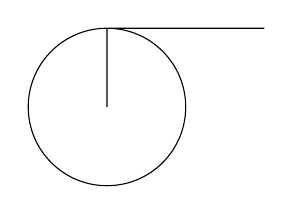
\begin{tikzpicture}
            \draw (0,0) circle[radius=1] |-(2,1);
        \end{tikzpicture}
    \end{adjustbox}
                     &
    \begin{adjustbox}{valign=t,minipage=\cwC}
        Move-To (0,0) (OR set current position to (0,0)), draw circle with current position as center and radius \qty{1}{\cm} (\textbf{current position is NOT moved}), then draw |- Line-To (2,1).
    \end{adjustbox}
    \\
    \tablerowseparatorline{}
    \begin{adjustbox}{valign=t,minipage=\cwA}
        \begin{lstlisting}[language={[LaTeX] TeX},numbers=none,frame=none,breaklines=true,aboveskip=0em,belowskip=0em,gobble=12,]
            \draw[->] (0,0) --(3.5,0);
            \draw[<-] (0,-1/2) --(3.5,-1/2);
        \end{lstlisting}
    \end{adjustbox}
                     &
    \begin{adjustbox}{valign=t,minipage=\cwB}
        \begin{tikzpicture}
            \draw[->] (0,0) --(3.5,0);
            \draw[<-] (0,-1/2) --(3.5,-1/2);
        \end{tikzpicture}
    \end{adjustbox}
                     &
    \begin{adjustbox}{valign=t,minipage=\cwC}
        \verb|\draw| の直後にオプション \texttt{[->]} や \texttt{[<-]} を書けば，その向きの矢印になる
    \end{adjustbox}
    \\
    \tablerowseparatorline{}
    \begin{adjustbox}{valign=t,minipage=\cwA}
        \begin{lstlisting}[language={[LaTeX] TeX},numbers=none,frame=none,breaklines=true,aboveskip=0em,belowskip=0em,gobble=12,]
            \draw[<->] (0,0) --(3.5,0);
            \draw[->>] (0,-1/2) --(3.5,-1/2);
            \draw[->,>=stealth] (0,-1) --(3.5,-1);
        \end{lstlisting}
    \end{adjustbox}
                     &
    \begin{adjustbox}{valign=t,minipage=\cwB}
        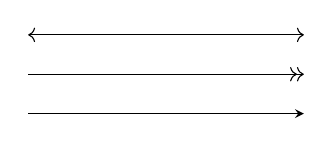
\begin{tikzpicture}
            \draw[<->] (0,0) --(3.5,0);
            \draw[->>] (0,-1/2) --(3.5,-1/2);
            \draw[->,>=stealth] (0,-1) --(3.5,-1);
        \end{tikzpicture}
    \end{adjustbox}
                     &
    \begin{adjustbox}{valign=t,minipage=\cwC}
        \texttt{[<->]} は両端点矢印で，\texttt{[->>]} は2重矢印で，\texttt{[->,>=stealth]} は stealth 機型矢印
    \end{adjustbox}
    \\
    \tablerowseparatorline{}
    \begin{adjustbox}{valign=t,minipage=\cwA}
        \begin{lstlisting}[language={[LaTeX] TeX},numbers=none,frame=none,breaklines=true,aboveskip=0em,belowskip=0em,gobble=12,]
            \draw[double distance=3pt,green,double=red] (0,0) --(3.5,0);
            \draw[ultra thick,blue] (0,-0.5) --(3.5,-0.5);
            \draw[double,->] (0,-1.0) --(3.5,-1.0);
            \draw[opacity=0.3] (0,-1.5) --(3.5,-1.5);
        \end{lstlisting}
    \end{adjustbox}
                     &
    \begin{adjustbox}{valign=t,minipage=\cwB}
        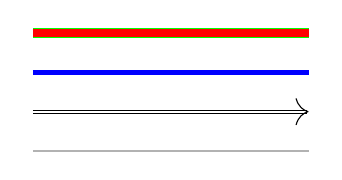
\begin{tikzpicture}
            \draw[double distance=3pt,green,double=red] (0,0) --(3.5,0);
            \draw[ultra thick,blue] (0,-0.5) --(3.5,-0.5);
            \draw[double,->] (0,-1.0) --(3.5,-1.0);
            \draw[opacity=0.3] (0,-1.5) --(3.5,-1.5);
        \end{tikzpicture}
    \end{adjustbox}
                     &
    \begin{adjustbox}{valign=t,minipage=\cwC}
        \verb|double distance=3pt,green| は緑色の，\qty{3}{pt} 離れる2重線で， \verb|double=red| はその間が赤色．
    \end{adjustbox}
    \\
    \tablerowseparatorline{}
    \begin{adjustbox}{valign=t,minipage=\cwA}
        \begin{lstlisting}[language={[LaTeX] TeX},numbers=none,frame=none,breaklines=true,aboveskip=0em,belowskip=0em,gobble=12,]
            \draw (0,0) --(0,2) (1,2) |-(2,0) --cycle;
        \end{lstlisting}
    \end{adjustbox}
                     &
    \begin{adjustbox}{valign=t,minipage=\cwB}
        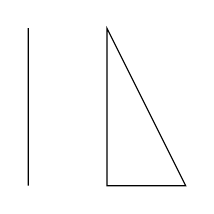
\begin{tikzpicture}
            \draw (0,0) --(0,2) (1,2) |-(2,0) --cycle;
        \end{tikzpicture}
    \end{adjustbox}
                     &
    \begin{adjustbox}{valign=t,minipage=\cwC}
        \verb|cycle| は直前の Move-To で指定した座標値．左のコマンドでは，最初の Move-To は (0,0) で，\verb|cycle| の直前の Move-To は (1,2) なので，\verb|cycle| は (1,2) の座標となる．
    \end{adjustbox}
    \\
    \tablerowseparatorline{}
    \begin{adjustbox}{valign=t,minipage=\cwA}
        \begin{lstlisting}[language={[LaTeX] TeX},numbers=none,frame=none,breaklines=true,aboveskip=0em,belowskip=0em,gobble=12,]
            \draw[ultra thick,orange] (0,0) --(3.5,0);
            \draw[ultra thick,red!60!blue] (0,-1.0) --(3.0,-1.0);
        \end{lstlisting}
    \end{adjustbox}
                     &
    \begin{adjustbox}{valign=t,minipage=\cwB}
        
\begin{tikzpicture}
            \draw[ultra thick,orange] (0,0) --(3.5,0);
            \draw[ultra thick,red!60!blue] (0,-1.0) --(3.0,-1.0);
        \end{tikzpicture}
    \end{adjustbox}
                     &
    \begin{adjustbox}{valign=t,minipage=\cwC}
        \texttt{[red!60!blue]} は赤色 \qty{60}{\percent}，残りは青色の混ぜ色
    \end{adjustbox}
    \\
    \addlinespace[0.3em]
\end{longtable}

表~\ref{tab:lineartransform}は図形の線形移動・拡大縮小・回転についてまとめる．リスト~\ref{lst:lineartranstemplate} は，表~\ref{tab:lineartransform} の線形移動などのためのテンプレートプログラムで，\verb|[shift={(1,2)},blue]| の様子を示す．
\begin{lstlisting}[
    language={[LaTeX] TeX},
    caption={図形線形移動・拡大縮小・回転のテンプレート},label={lst:lineartranstemplate},
    firstnumber=1,breaklines=true,gobble=4]
    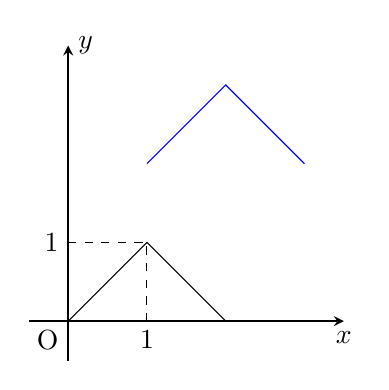
\begin{tikzpicture}
        \draw[->,>=stealth,semithick] (-0.5,0) --(3.5,0) node[below]{$x$}; %x軸
        \draw[->,>=stealth,semithick] (0,-0.5) --(0,3.5) node[right]{$y$}; %y軸
        \draw (0,0) node[below left]{O}; %原点
        \draw[dashed] (1,0) node[below]{1} --(1,1) --(0,1) node[left]{1}; %点(1,1)
        \draw (0,0) --(1,1) --(2,0); %移動前
        \draw[shift={(1,2)},blue] (0,0) --(1,1) --(2,0); %移動後
    \end{tikzpicture}
\end{lstlisting}

\[
    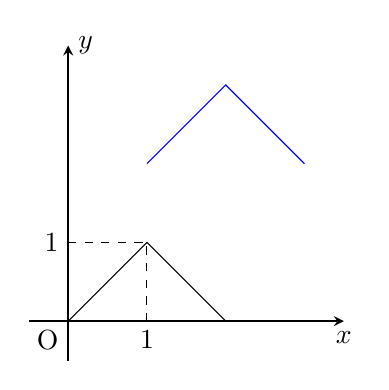
\begin{tikzpicture}
    \draw[->,>=stealth,semithick] (-0.5,0) --(3.5,0) node[below]{$x$}; %x軸
    \draw[->,>=stealth,semithick] (0,-0.5) --(0,3.5) node[right]{$y$}; %y軸
    \draw (0,0) node[below left]{O}; %原点
    \draw[dashed] (1,0) node[below]{1} --(1,1) --(0,1) node[left]{1}; %点(1,1)
    \draw (0,0) --(1,1) --(2,0); %移動前
    \draw[shift={(1,2)},blue] (0,0) --(1,1) --(2,0); %移動後
    \end{tikzpicture}
\]

\newcommand{\cwD}{9cm}
\newcommand{\cwE}{6cm}
\newcommand{\twocolrowseparatorline}{
    \addlinespace[0.3em]
    \cmidrule{1-2}
    \addlinespace[0.2em]
}
\begin{longtable}{p{\cwD} p{\cwE}}
    \caption{図形の線形移動・拡大縮小・回転のオプションと出力} \label{tab:lineartransform}                      \\[-1em]
    \toprule
    \textbf{Command} & \textbf{Rendered Output}                                         \\
    \midrule
    \endfirsthead % chktex 1

    % \midrule
    \multicolumn{2}{c}{表~\ref{tab:lineartransform}:~\nameref{tab:lineartransform}（の続き）} \\[0.3em]
    \toprule
    \textbf{Command} & \textbf{Rendered Output}                                         \\
    \midrule
    \endhead % chktex 1

    % \midrule
    \multicolumn{2}{r}{表~\ref{tab:lineartransform}（次のページへ続く）}                           \\
    \midrule
    \endfoot % chktex 1

    \midrule
    \multicolumn{2}{r}{表~\ref{tab:lineartransform}終了}                                   \\
    \bottomrule
    \endlastfoot % chktex 1

    \begin{adjustbox}{valign=t,minipage=\cwD}
        \begin{lstlisting}[language={[LaTeX] TeX},numbers=none,frame=none,breaklines=true,aboveskip=0em,belowskip=0em,gobble=12,]
            \draw[scale=2,blue] (0,0) --(1,1) --(2,0);
        \end{lstlisting}
    \end{adjustbox}
                     &
    \begin{adjustbox}{valign=t,minipage=\cwE}
        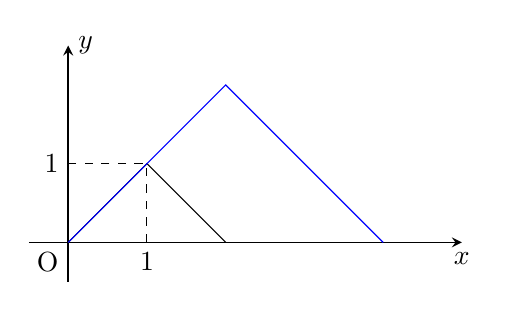
\begin{tikzpicture}
            \draw[->,>=stealth,semithick] (-0.5,0) --(5,0) node[below]{$x$}; %x軸
            \draw[->,>=stealth,semithick] (0,-0.5) --(0,2.5) node[right]{$y$}; %y軸
            \draw (0,0) node[below left]{O}; %原点
            \draw[dashed] (1,0) node[below]{1} --(1,1) --(0,1) node[left]{1}; %点(1,1)
            \draw (0,0) --(1,1) --(2,0); %移動前
            \draw[scale=2,blue] (0,0) --(1,1) --(2,0);
        \end{tikzpicture}
    \end{adjustbox}
    \\
    \twocolrowseparatorline{}
    \begin{adjustbox}{valign=t,minipage=\cwD}
        \begin{lstlisting}[language={[LaTeX] TeX},numbers=none,frame=none,breaklines=true,aboveskip=0em,belowskip=0em,gobble=12,]
            \draw[scale around={2:(2.0,1.5)},blue] (0,0) --(1,1) --(2,0);
            \node[circle, fill, inner sep=1pt] at (2.0,1.5) {};
        \end{lstlisting}
    \end{adjustbox}
                     &
    \begin{adjustbox}{valign=t,minipage=\cwE}
        \begin{tikzpicture}
            \draw[->,>=stealth,semithick] (-2.5,0) --(3.0,0) node[below]{$x$}; %x軸
            \draw[->,>=stealth,semithick] (0,-2.0) --(0,2.0) node[right]{$y$}; %y軸
            \draw (0,0) node[below left]{O}; %原点
            \draw[dashed] (1,0) node[below]{1} --(1,1) --(0,1) node[left]{1}; %点(1,1)
            \draw (0,0) --(1,1) --(2,0); %移動前
            \draw[scale around={2:(2.0,1.5)},blue] (0,0) --(1,1) --(2,0);
            \node[circle, fill, inner sep=1pt] at (2.0,1.5) {};
        \end{tikzpicture}
    \end{adjustbox}
    \\
    \twocolrowseparatorline{}
    \begin{adjustbox}{valign=t,minipage=\cwD}
        \begin{lstlisting}[language={[LaTeX] TeX},numbers=none,frame=none,breaklines=true,aboveskip=0em,belowskip=0em,gobble=12,]
            \draw[rotate=20,blue] (0,0) --(1,1) --(2,0);
        \end{lstlisting}
    \end{adjustbox}
                     &
    \begin{adjustbox}{valign=t,minipage=\cwE}
        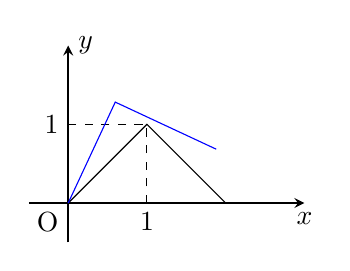
\begin{tikzpicture}
            \draw[->,>=stealth,semithick] (-0.5,0) --(3,0) node[below]{$x$}; %x軸
            \draw[->,>=stealth,semithick] (0,-0.5) --(0,2.0) node[right]{$y$}; %y軸
            \draw (0,0) node[below left]{O}; %原点
            \draw[dashed] (1,0) node[below]{1} --(1,1) --(0,1) node[left]{1}; %点(1,1)
            \draw (0,0) --(1,1) --(2,0); %移動前
            \draw[rotate=20,blue] (0,0) --(1,1) --(2,0);
        \end{tikzpicture}
    \end{adjustbox}
    \\
    \twocolrowseparatorline{}
    \begin{adjustbox}{valign=t,minipage=\cwD}
        \begin{lstlisting}[language={[LaTeX] TeX},numbers=none,frame=none,breaklines=true,aboveskip=0em,belowskip=0em,gobble=12,]
            \draw[rotate around={20:(1,1)},blue] (0,0) --(1,1) --(2,0);
        \end{lstlisting}
    \end{adjustbox}
                     &
    \begin{adjustbox}{valign=t,minipage=\cwE}
        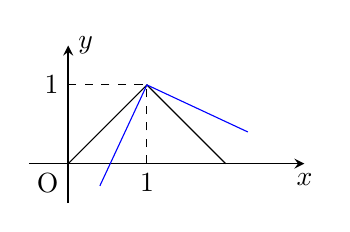
\begin{tikzpicture}
            \draw[->,>=stealth,semithick] (-0.5,0) --(3,0) node[below]{$x$}; %x軸
            \draw[->,>=stealth,semithick] (0,-0.5) --(0,1.5) node[right]{$y$}; %y軸
            \draw (0,0) node[below left]{O}; %原点
            \draw[dashed] (1,0) node[below]{1} --(1,1) --(0,1) node[left]{1}; %点(1,1)
            \draw (0,0) --(1,1) --(2,0); %移動前
            \draw[rotate around={20:(1,1)},blue] (0,0) --(1,1) --(2,0);
        \end{tikzpicture}
    \end{adjustbox}
    \\
    \twocolrowseparatorline{}
    \begin{adjustbox}{valign=t,minipage=\cwD}
        \begin{lstlisting}[language={[LaTeX] TeX},numbers=none,frame=none,breaklines=true,aboveskip=0em,belowskip=0em,gobble=12,]
            \draw[rotate around={-30:(2.0,1.5)},blue] (0,0) --(1,1) --(2,0);
            \node[circle, fill, inner sep=1pt] at (2.0,1.5) {};
        \end{lstlisting}
    \end{adjustbox}
                     &
    \begin{adjustbox}{valign=t,minipage=\cwE}
        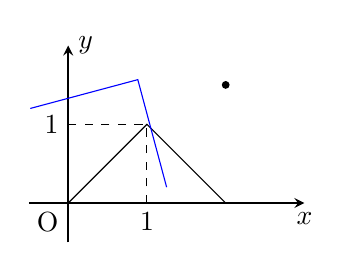
\begin{tikzpicture}
            \draw[->,>=stealth,semithick] (-0.5,0) --(3,0) node[below]{$x$}; %x軸
            \draw[->,>=stealth,semithick] (0,-0.5) --(0,2.0) node[right]{$y$}; %y軸
            \draw (0,0) node[below left]{O}; %原点
            \draw[dashed] (1,0) node[below]{1} --(1,1) --(0,1) node[left]{1}; %点(1,1)
            \draw (0,0) --(1,1) --(2,0); %移動前
            \draw[rotate around={-30:(2.0,1.5)},blue] (0,0) --(1,1) --(2,0);
            \node[circle, fill, inner sep=1pt] at (2.0,1.5) {};
        \end{tikzpicture}
    \end{adjustbox}
    \\
    \addlinespace[0.3em]
\end{longtable}

\section{「\LaTeX{}で図を直接描けるTikZの使い方３｜グラフの描き方」}
\label{plotgraph}

第~\ref{plotgraph}章では，\url{https://math-note.xyz/latex/tikz/tikz-graph/}にあるコードを，いくつか試してみる．

リスト~\ref{lst:plotgraph} は，関数 \(y=x+1 \) の関数のグラフを示す．
\begin{lstlisting}[
    language={[LaTeX] TeX},
    caption={関数・グラフを plot するテンプレート},label={lst:plotgraph},
    firstnumber=1,breaklines=true,gobble=4]
    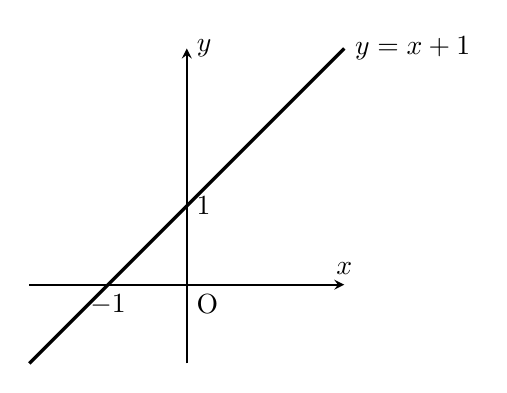
\begin{tikzpicture}
        \draw[->,>=stealth,semithick] (-2,0)--(2,0) node[above]{$x$}; %x軸
        \draw[->,>=stealth,semithick] (0,-1)--(0,3) node[right]{$y$}; %y軸
        \draw (0,0) node[below right]{O}; %原点
        \draw (-1,0) node[below]{$-1$}; %点(-1,0)
        \draw (0,1) node[right]{$1$}; %点(0,1)
        \draw[very thick,domain=-2:2] plot(\x,\x+1) node[right]{$y=x+1$}; %y=x+1のグラフ
    \end{tikzpicture}
\end{lstlisting}

\[
    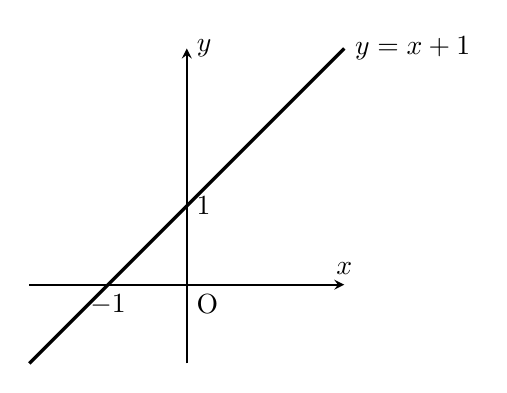
\begin{tikzpicture}
    \draw[->,>=stealth,semithick] (-2,0)--(2,0) node[above]{$x$}; %x軸
    \draw[->,>=stealth,semithick] (0,-1)--(0,3) node[right]{$y$}; %y軸
    \draw (0,0) node[below right]{O}; %原点
    \draw (-1,0) node[below]{$-1$}; %点(-1,0)
    \draw (0,1) node[right]{$1$}; %点(0,1)
    \draw[very thick,domain=-2:2] plot(\x,\x+1) node[right]{$y=x+1$}; %y=x+1のグラフ
    \end{tikzpicture}
\]

ネイピア数 \(e \) は \verb|e| で，円周率 \(\pi \) は \verb|pi| で書く．

TikZ で関数のグラフを描くときは，以下に注意：
\begin{description}
    \item[Default変数は \texttt{\textbackslash x}] 媒介変数 (parametric plot) を行いたいとき，オプション \verb|[variable=\t]| を追加 % chktex 1
    \item[関数は \{と \}との間に囲む] \verb|\draw[domain=0:2.5] plot(\x,sqrt(\x));| はエラーで，\\
          \verb|\draw[domain=0:2.5] plot(\x,{sqrt(\x)});| で入力すべき
    \item[radian は明示的に指定] \verb|\draw(pi,{sin(pi)}) node{A};| とすると，点 (\(\pi, \sin \qty[parse-numbers=false]{\pi}{\degree}\)) に \(A \) が表示されてしまう．\verb|\draw(pi,{sin(pi r)}) node{A};| で入力すべき
\end{description}

以下の通り記述すれば，
\begin{lstlisting}[
    language={[LaTeX] TeX},
    firstnumber=1,breaklines=true,gobble=4]
    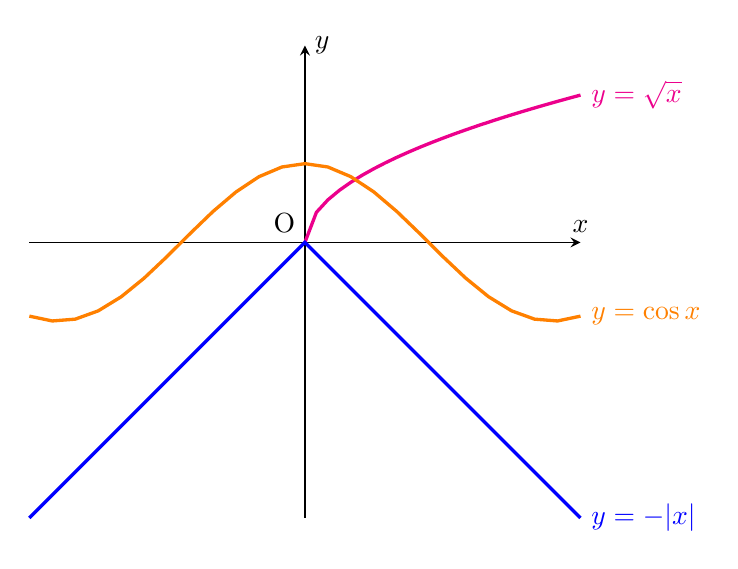
\begin{tikzpicture}
        \draw[->,>=stealth,semithick] (-3.5,0)--(3.5,0) node[above]{$x$}; %x軸
        \draw[->,>=stealth,semithick] (0,-3.5)--(0,2.5) node[right]{$y$}; %y軸
        \draw (0,0) node[above left]{O}; %原点
        \draw[magenta,very thick,domain=0:3.5] plot(\x,{sqrt(\x)}) node[right]{$y=\sqrt{x}$};
        \draw[blue,very thick,domain=-3.5:3.5] plot(\x,{-abs(\x)}) node[right]{$y=-|x|$};
        \draw[orange,very thick,domain=-3.5:3.5] plot(\x,{cos(\x r)}) node[right]{$y=\cos{x}$};
    \end{tikzpicture}
\end{lstlisting}
以下のグラフが得られる．
\[
    \begin{tikzpicture}
    \draw[->,>=stealth,semithick] (-3.5,0)--(3.5,0) node[above]{$x$}; %x軸
    \draw[->,>=stealth,semithick] (0,-3.5)--(0,2.5) node[right]{$y$}; %y軸
    \draw (0,0) node[above left]{O}; %原点
    \draw[magenta,very thick,domain=0:3.5] plot(\x,{sqrt(\x)}) node[right]{$y=\sqrt{x}$};
    \draw[blue,very thick,domain=-3.5:3.5] plot(\x,{-abs(\x)}) node[right]{$y=-|x|$};
    \draw[orange,very thick,domain=-3.5:3.5] plot(\x,{cos(\x r)}) node[right]{$y=\cos{x}$};
    \end{tikzpicture}
\]

\subsection{プロットする点を増やす方法}

オプション \verb|[samples=100,domain=0:2.5]| で，\verb|\x| のサンプル数を 100 にする．
\begin{lstlisting}[
    language={[LaTeX] TeX},
    firstnumber=1,breaklines=true,gobble=4]
    \begin{tikzpicture}
        \draw[->,>=stealth,semithick] (-3.5,0)--(3.5,0) node[above]{$x$}; %x軸
        \draw[->,>=stealth,semithick] (0,-3.5)--(0,2.5) node[right]{$y$}; %y軸
        \draw (0,0) node[above left]{O}; %原点
        \draw[magenta,very thick,samples=100,domain=0:3.5] plot(\x,{sqrt(\x)}) node[right]{$y=\sqrt{x}$};
        \draw[blue,very thick,domain=-3.5:3.5] plot(\x,{-abs(\x)}) node[right]{$y=-|x|$};
        \draw[orange,very thick,samples=100,domain=-3.5:3.5] plot(\x,{cos(\x r)}) node[right]{$y=\cos{x}$};
    \end{tikzpicture}
\end{lstlisting}
\[
    \begin{tikzpicture}
    \draw[->,>=stealth,semithick] (-3.5,0)--(3.5,0) node[above]{$x$}; %x軸
    \draw[->,>=stealth,semithick] (0,-3.5)--(0,2.5) node[right]{$y$}; %y軸
    \draw (0,0) node[above left]{O}; %原点
    \draw[magenta,very thick,samples=100,domain=0:3.5] plot(\x,{sqrt(\x)}) node[right]{$y=\sqrt{x}$};
    \draw[blue,very thick,domain=-3.5:3.5] plot(\x,{-abs(\x)}) node[right]{$y=-|x|$};
    \draw[orange,very thick,samples=100,domain=-3.5:3.5] plot(\x,{cos(\x r)}) node[right]{$y=\cos{x}$};
    \end{tikzpicture}
\]

\subsection{変数を変える方法・parametric plot}

オプション \verb|[variable=\t]| で，default の \verb|\x| の代わりに \verb|\t| を媒介変数 (parameter) として使う．
\begin{lstlisting}[
    language={[LaTeX] TeX},
    firstnumber=1,breaklines=true,gobble=4]
    \begin{tikzpicture}
        \draw[->,>=stealth,semithick] (-0.5,0)--(2*pi+0.5,0) node[above]{$x$}; %x軸
        \draw[->,>=stealth,semithick] (0,-0.5)--(0,2.5) node[right]{$y$}; %y軸
        \draw (0,0) node[above left]{O}; %原点
        \draw[very thick,samples=100,domain=0:2*pi,variable=\t] plot({\t-sin(\t r)},{1-cos(\t r)}); %サイクロイド
        \draw (2*pi,0) node[below]{$2 \pi$}; %点(2 \pi,0)
        \draw[dashed] (0,2) node[left]{2}--(pi,2)--(pi,0) node[below]{$\pi$}; %点(\pi,2)
    \end{tikzpicture}
\end{lstlisting}
\[
    \begin{tikzpicture}
    \draw[->,>=stealth,semithick] (-0.5,0)--(2*pi+0.5,0) node[above]{$x$}; %x軸
    \draw[->,>=stealth,semithick] (0,-0.5)--(0,2.5) node[right]{$y$}; %y軸
    \draw (0,0) node[above left]{O}; %原点
    \draw[very thick,samples=100,domain=0:2*pi,variable=\t] plot({\t-sin(\t r)},{1-cos(\t r)}); %サイクロイド
    \draw (2*pi,0) node[below]{$2 \pi$}; %点(2 \pi,0)
    \draw[dashed] (0,2) node[left]{2}--(pi,2)--(pi,0) node[below]{$\pi$}; %点(\pi,2)
    \end{tikzpicture}
\]

\subsection{極座標の基本の描き方}

極座標上の偏角 \(\qty[parse-numbers=false]{a}{\degree} \)，半径 \(r \) の点 \((\qty[parse-numbers=false]{a}{\degree}, r)\) は，TikZ では \verb|(a:r)| で表す．例えば，\verb|\draw[->] (0,0) --(30:2cm);| は，
\(
\begin{tikzpicture}
    \draw[->] (0,0) --(30:2cm);
\end{tikzpicture}
\)
と表示される．

弧度法 (radian) として解釈させたい場合は，\verb|r| を付ける．例えば，\verb|\draw[->] (0,0) --(pi/4 r:2cm);| は，
\(
\begin{tikzpicture}
    \draw[->] (0,0) --(pi/4 r:2cm);
\end{tikzpicture}
\)
と表示される．

\subsection{\texttt{++} による相対的 Move-To}

\verb|(a,b)| は，現在地を絶対的に \verb|(a,b)| に Move-To する．\verb|++(c,d)| は現在地に対して相対的に \verb|(c,d)| 分だけ移動して，新しい現在地を \verb|(a+c,b+d)| にする．

極座標表現でももちろん使える．つまり \verb|++(e:r)| とした場合，新しい現在地は \((a+r \cos e, b+r \sin e) \)となる．

\subsection{極座標での円弧 (arc) の描き方}

半径 \(r \) の円に対して，偏角 \(\qty[parse-numbers=false]{a}{\degree}\) の位置にある点 \verb|(A)| と 偏角 \(\qty[parse-numbers=false]{b}{\degree}\) の位置にある点 \verb|B| を考える．

この弧 (arc) AB は， \verb|\draw (A) arc(a:b:r);| と記述すれば表示できる．

例えば，
\begin{lstlisting}[
    language={[LaTeX] TeX},
    firstnumber=1,breaklines=true,gobble=4]
    \begin{tikzpicture}
        \draw[->,>=stealth,semithick] (-1.5,0) --(2.5,0) node[above]{$x$}; %x軸
        \draw[->,>=stealth,semithick] (0,-0.5) --(0,2) node[right]{$y$}; %y軸
        \draw (0,0) node[above left]{O}; %原点
        \draw (2,1) node[right]{A}; %点A(2,1)
        \draw[very thick] (2,1) arc (60:110:3cm); %点Aが偏角60度の点であるような半径3の円の，偏角60度から110度の部分の円弧
        \draw (2,1) ++(60:-3) ++(110:3) node[left]{B}; %円弧のAでない方の端点B(2,1)
    \end{tikzpicture}
\end{lstlisting}
と記述すれば，
\[
    \begin{tikzpicture}
    \draw[->,>=stealth,semithick] (-1.5,0) --(2.5,0) node[above]{$x$}; %x軸
    \draw[->,>=stealth,semithick] (0,-0.5) --(0,2) node[right]{$y$}; %y軸
    \draw (0,0) node[above left]{O}; %原点
    \draw (2,1) node[right]{A}; %点A(2,1)
    \draw[very thick] (2,1) arc (60:110:3cm); %点Aが偏角60度の点であるような半径3の円の，偏角60度から110度の部分の円弧
    \draw (2,1) ++(60:-3) ++(110:3) node[left]{B}; %円弧のAでない方の端点B(2,1)
    \end{tikzpicture}
\]
と表示される．

\subsection{極方程式のグラフの描き方}

例えば，\(a > 0 \) に対して極方程式 \(r=2a \cos \theta \) は，\verb|plot(\theta r:{2*a*cos(\theta r)})| を使って，以下のように
\begin{lstlisting}[
    language={[LaTeX] TeX},
    firstnumber=1,breaklines=true,gobble=4]
    \begin{tikzpicture}
        \draw[->,>=stealth,semithick] (0,0)--(4,0) node[right]{$x$}; %始線
        \draw (0,0) node[left]{O}; %極
        \draw[very thick,samples=100,domain=0:pi,variable=\theta] plot(\theta r:{2*1.5*cos(\theta r)}); %点(1.5,0)を中心とする半径1.5の円
    \end{tikzpicture}
\end{lstlisting}
記述すれば，
\[
    \begin{tikzpicture}
    \draw[->,>=stealth,semithick] (0,0)--(4,0) node[right]{$x$}; %始線
    \draw (0,0) node[left]{O}; %極
    \draw[very thick,samples=100,domain=0:pi,variable=\theta] plot(\theta r:{2*1.5*cos(\theta r)}); %点(1.5,0)を中心とする半径1.5の円
    \end{tikzpicture}
\]
と極座標上で点 (1.5,0) を中心とする半径 1.5 の円が表示される．

\section{「\LaTeX{}で図を直接描けるTikZの使い方４｜座標の定義と計算」}
\label{coordinatedefcalc}

第~\ref{coordinatedefcalc}章では，\url{https://math-note.xyz/latex/tikz/tikz-coordinate/}にあるコードを，いくつか試してみる．

\subsection{How to define a coordinate point as variable, assign label to it, and draw mark on it}

変数である点 \verb|(A)| を，座標 \verb|(0,0)| として定義して，``Point A'' として \qty{200}{\degree} にラベルを付けるには，以下のようにする．ただし，点は表示できないから，ラベルである ``Point A'' だけが表示されることになる．

\begin{lstlisting}[
    language={[LaTeX] TeX},
    firstnumber=1,breaklines=true,gobble=4]
    \begin{tikzpicture}
        \coordinate[label=200:Point A] (A) at (0,0);
    \end{tikzpicture}
\end{lstlisting}
\[
    \begin{tikzpicture}
        \coordinate[label=200:Point A] (A) at (0,0);
    \end{tikzpicture}
\]

その点 \verb|(A)| を表示するには，mark として小さな circle または rectangle を書いても良い．
\begin{lstlisting}[
    language={[LaTeX] TeX},
    firstnumber=1,breaklines=true,gobble=4]
    \begin{tikzpicture}
        \coordinate[label=200:Point A] (A) at (0,0);
        \fill[red] (A) circle[radius=0.06cm];
    \end{tikzpicture}
\end{lstlisting}
\[
    \begin{tikzpicture}
        \coordinate[label=200:Point A] (A) at (0,0);
        \fill[red] (A) circle[radius=0.06cm];
    \end{tikzpicture}
\]
\begin{lstlisting}[
    language={[LaTeX] TeX},
    firstnumber=1,breaklines=true,gobble=4]
    \begin{tikzpicture}
        \coordinate[label=200:Point A] (A) at (0,0);
        \fill[cyan] (A) +(-0.06,-0.06) rectangle +(0.06,0.06);
    \end{tikzpicture}
\end{lstlisting}
\[
    \begin{tikzpicture}
        \coordinate[label=200:Point A] (A) at (0,0);
        \fill[cyan] (A) +(-0.06,-0.06) rectangle +(0.06,0.06);
    \end{tikzpicture}
\]

以下の例では，まず３点 \verb|(A), (B), (C)| の座標値を定義して，それぞれ ``Point A''，``Point B''，``Point C'' という label （とその label の位置）をつける．それから \verb|(A), (B), (C)| を頂点とする三角形を描く．この例では，頂点 \verb|(A), (B), (C)| に mark が描かれていないことに注意．
\begin{lstlisting}[
    language={[LaTeX] TeX},
    firstnumber=1,breaklines=true,gobble=4]
    \begin{tikzpicture}
        \coordinate[label=200:Point A] (A) at (0,0);
        \coordinate[label=-20:Point B] (B) at (3,0);
        \coordinate[label=above:Point C] (C) at (2,2);
        \draw (A) --(B) --(C) --cycle;
    \end{tikzpicture}
\end{lstlisting}
\[
    \begin{tikzpicture}
        \coordinate[label=200:Point A] (A) at (0,0);
        \coordinate[label=-20:Point B] (B) at (3,0);
        \coordinate[label=above:Point C] (C) at (2,2);
        \draw (A) --(B) --(C) --cycle;
    \end{tikzpicture}
\]

以下の例では，上記の３つの頂点に mark を付ける方法を示す．各頂点に一つずつ \verb|fill[]| をしないで，\verb|\foreach| で頂点の分だけ繰り返し mark を付ける．
\begin{lstlisting}[
    language={[LaTeX] TeX},
    firstnumber=1,breaklines=true,gobble=4]
    \begin{tikzpicture}
        \coordinate[label=200:Point A] (A) at (0,0);
        \coordinate[label=-20:Point B] (B) at (3,0);
        \coordinate[label=above:Point C] (C) at (2,2);
        \foreach \P in {A,B,C} \fill[cyan] (\P) circle[radius=0.06cm];
        \draw (A) --(B) --(C) --cycle;
    \end{tikzpicture}
\end{lstlisting}
\[
    \begin{tikzpicture}
        \coordinate[label=200:Point A] (A) at (0,0);
        \coordinate[label=-20:Point B] (B) at (3,0);
        \coordinate[label=above:Point C] (C) at (2,2);
        \foreach \P in {A,B,C} \fill[cyan] (\P) circle[radius=0.06cm];
        \draw (A) --(B) --(C) --cycle;
    \end{tikzpicture}
\]

\subsection{Define and give a name to intersection of paths}

By default, the name of intersection is \verb|intersection-1|, \verb|intersection-2|, etc.
\begin{lstlisting}[
    language={[LaTeX] TeX},
    firstnumber=1,breaklines=true,gobble=4]
    \begin{tikzpicture}
        \draw[name path=C1] (0,0) circle[radius=1]; %円C1
        \draw[name path=C2] (2,1) circle[radius=2]; %円C2
        \path[name intersections={of=C1 and C2}]; %円C1と円C2の交点の定義
        \fill[blue] (intersection-1) circle[radius=0.06] node[above left]{A}; %1つ目の交点の左にA
        \fill[magenta] (intersection-2) circle[radius=0.06] node[below]{B}; %2つ目の交点の下にB
    \end{tikzpicture}
\end{lstlisting}
\[
    \begin{tikzpicture}
        \draw[name path=C1] (0,0) circle[radius=1]; %円C1
        \draw[name path=C2] (2,1) circle[radius=2]; %円C2
        \path[name intersections={of=C1 and C2}]; %円C1と円C2の交点の定義
        \fill[blue] (intersection-1) circle[radius=0.06] node[above left]{A}; %1つ目の交点の左にA
        \fill[magenta] (intersection-2) circle[radius=0.06] node[below]{B}; %2つ目の交点の下にB
    \end{tikzpicture}
\]

Using keyword \verb|name by|, we can name the intersection as we like. Notice that we can also assign variable name to a path using \verb|name| (\verb|C1| and \verb|C2|).
\begin{lstlisting}[
    language={[LaTeX] TeX},
    firstnumber=1,breaklines=true,gobble=4]
    \begin{tikzpicture}
        \draw[name path=C1] (0,0) circle[radius=1]; %円C1
        \draw[name path=C2] (2,1) circle[radius=2]; %円C2
        \path[name intersections={of=C1 and C2, by={A}}]; %Just name 1 intersection only: A
        \fill[blue] (A) circle[radius=0.06] node[above left]{Point A};
        \fill[magenta] (intersection-2) circle[radius=0.06] node[right]{Point B};
        % \path[name intersections={of=C1 and C2, by={A,B}}]; %OR like this, name both intersections as A,B
        % \fill[blue] (A) circle[radius=0.06] node[above left]{Point A}; %1つ目の交点の左にA
        % \fill[magenta] (B) circle[radius=0.06] node[right]{Point B}; %2つ目の交点の下にB
    \end{tikzpicture}
\end{lstlisting}
\[
    \begin{tikzpicture}
        \draw[name path=C1] (0,0) circle[radius=1]; %円C1
        \draw[name path=C2] (2,1) circle[radius=2]; %円C2
        \path[name intersections={of=C1 and C2, by={A}}]; %Just name 1 intersection only: A
        \fill[blue] (A) circle[radius=0.06] node[above left]{Point A};
        \fill[magenta] (intersection-2) circle[radius=0.06] node[right]{Point B};
        % \path[name intersections={of=C1 and C2, by={A,B}}]; %OR like this, name both intersections as A,B
        % \fill[blue] (A) circle[radius=0.06] node[above left]{Point A}; %1つ目の交点の左にA
        % \fill[magenta] (B) circle[radius=0.06] node[right]{Point B}; %2つ目の交点の下にB
    \end{tikzpicture}
\]

\subsection{座標の計算 (Performing Calculation on Coordinates)}

\subsubsection{利用できる座標の計算}

表~\ref{tab:calccoord}は，点の座標計算（和・スカラー倍・内分・外分・垂線の足など）をまとめる．

\renewcommand{\cwD}{11cm}
\renewcommand{\cwE}{4.5cm}
\begin{longtable}{p{\cwD} p{\cwE}}
    \caption{TikZ の座標計算} \label{tab:calccoord}                              \\[-1em]
    \toprule
    \textbf{Command} & \textbf{Rendered Output}                             \\
    \midrule
    \endfirsthead % chktex 1

    % \midrule
    \multicolumn{2}{c}{表~\ref{tab:calccoord}:~\nameref{tab:calccoord}（の続き）} \\[0.3em]
    \toprule
    \textbf{Command} & \textbf{Rendered Output}                             \\
    \midrule
    \endhead % chktex 1

    % \midrule
    \multicolumn{2}{r}{表~\ref{tab:calccoord}（次のページへ続く）}                     \\
    \midrule
    \endfoot % chktex 1

    \midrule
    \multicolumn{2}{r}{表~\ref{tab:calccoord}終了}                             \\
    \bottomrule
    \endlastfoot % chktex 1

    \begin{adjustbox}{valign=t,minipage=\cwD}
        \begin{lstlisting}[language={[LaTeX] TeX},numbers=none,frame=none,breaklines=true,aboveskip=0em,belowskip=0em,gobble=12,]
            % Addition ($(A)+(B)$)
            \coordinate (A) at (1.5,0.5);
            \coordinate (B) at (1,1.5);
            \draw[dashed, ->] (0,0) --(A) node[below right=-0.1cm]{A};
            \draw[dashed, ->] (0,0) --(B) node[above left=0cm]{B};
            \draw[->] (0,0) --($(A)+(B)$) node[right]{A+B};
        \end{lstlisting}
    \end{adjustbox}
                     &
    \begin{adjustbox}{valign=t,minipage=\cwE}
        \begin{tikzpicture}
            % Addition ($(A)+(B)$)
            \coordinate (A) at (1.5,0.5);
            \coordinate (B) at (1,1.5);
            \draw[dashed, ->] (0,0) --(A) node[below right=-0.1cm]{A};
            \draw[dashed, ->] (0,0) --(B) node[above left=0cm]{B};
            \draw[->] (0,0) --($(A)+(B)$) node[right]{A+B};
        \end{tikzpicture}
    \end{adjustbox}
    \\
    \twocolrowseparatorline{}
    \begin{adjustbox}{valign=t,minipage=\cwD}
        \begin{lstlisting}[language={[LaTeX] TeX},numbers=none,frame=none,breaklines=true,aboveskip=0em,belowskip=0em,gobble=12,]
            % Scale ($k*(A)$)
            \coordinate (A) at (1.5,0.5);
            \draw[cyan, ultra thick, ->] (0,0) --(A) node[above left=0.1cm]{A};
            \draw[thin, ->] (0,0) --($2*(A)$) node[above left]{2*A};
        \end{lstlisting}
    \end{adjustbox}
                     &
    \begin{adjustbox}{valign=t,minipage=\cwE}
        \begin{tikzpicture}
            % Scale ($k*(A)$)
            \coordinate (A) at (1.5,0.5);
            \draw[cyan, ultra thick, ->] (0,0) --(A) node[above left=0.1cm]{A};
            \draw[thin, ->] (0,0) --($2*(A)$) node[above left]{2*A};
        \end{tikzpicture}
    \end{adjustbox}
    \\
    \twocolrowseparatorline{}
    \begin{adjustbox}{valign=t,minipage=\cwD}
        \begin{lstlisting}[language={[LaTeX] TeX},numbers=none,frame=none,breaklines=true,aboveskip=0em,belowskip=0em,gobble=12,]
            % ($(A)!t!(B)$): 線分ABの内分点 (0<t<1)
            \coordinate[label=160:A] (A) at (0,0);
            \coordinate[label=-20:B] (B) at (3,2);
            \draw[very thin] (A) --(B);
            \coordinate[label=above left:(\$(A)!0.7!(B)\$)] (T) at ($(A)!0.7!(B)$);
            \foreach \P in {A,B} \fill[cyan] (\P) circle[radius=0.06cm];
            \fill[red] (T) +(-0.06,-0.06) rectangle +(0.06,0.06);
        \end{lstlisting}
    \end{adjustbox}
                     &
    \begin{adjustbox}{valign=t,minipage=\cwE}
        \begin{tikzpicture}
            % ($(A)!t!(B)$): 線分ABの内分点 (0<t<1)
            \coordinate[label=160:A] (A) at (0,0);
            \coordinate[label=-20:B] (B) at (3,2);
            \draw[very thin] (A) --(B);
            \coordinate[label=above left:(\$(A)!0.7!(B)\$)] (T) at ($(A)!0.7!(B)$);
            \foreach \P in {A,B} \fill[cyan] (\P) circle[radius=0.06cm];
            \fill[red] (T) +(-0.06,-0.06) rectangle +(0.06,0.06);
        \end{tikzpicture}
    \end{adjustbox}
    \\
    \twocolrowseparatorline{}
    \begin{adjustbox}{valign=t,minipage=\cwD}
        \begin{lstlisting}[language={[LaTeX] TeX},numbers=none,frame=none,breaklines=true,aboveskip=0em,belowskip=0em,gobble=12,]
            % ($(A)!t!(B)$): 線分ABの外分点 (t<0)
            \coordinate[label=right:A] (A) at (0,0);
            \coordinate[label=right:B] (B) at (0.5,2);
            \draw[very thin] (A) --(B);
            \coordinate[label=left:(\$(A)!-0.4!(B)\$)] (T) at ($(A)!-0.4!(B)$);
            \foreach \P in {A,B} \fill[cyan] (\P) circle[radius=0.06cm];
            \fill[red] (T) +(-0.06,-0.06) rectangle +(0.06,0.06);
        \end{lstlisting}
    \end{adjustbox}
                     &
    \begin{adjustbox}{valign=t,minipage=\cwE}
        \begin{tikzpicture}
            % ($(A)!t!(B)$): 線分ABの外分点 (t<0)
            \coordinate[label=right:A] (A) at (0,0);
            \coordinate[label=right:B] (B) at (0.5,2);
            \draw[very thin] (A) --(B);
            \coordinate[label=left:(\$(A)!-0.4!(B)\$)] (T) at ($(A)!-0.4!(B)$);
            \foreach \P in {A,B} \fill[cyan] (\P) circle[radius=0.06cm];
            \fill[red] (T) +(-0.06,-0.06) rectangle +(0.06,0.06);
        \end{tikzpicture}
    \end{adjustbox}
    \\
    \twocolrowseparatorline{}
    \begin{adjustbox}{valign=t,minipage=\cwD}
        \begin{lstlisting}[language={[LaTeX] TeX},numbers=none,frame=none,breaklines=true,aboveskip=0em,belowskip=0em,gobble=12,]
            % ($(A)!t!(B)$): 線分ABの外分点 (1<t)
            \coordinate[label=right:A] (A) at (0,0);
            \coordinate[label=right:B] (B) at (0.5,2);
            \draw[very thin] (A) --(B);
            \coordinate[label=left:(\$(A)!1.4!(B)\$)] (T) at ($(A)!1.4!(B)$);
            \foreach \P in {A,B} \fill[cyan] (\P) circle[radius=0.06cm];
            \fill[red] (T) +(-0.06,-0.06) rectangle +(0.06,0.06);
        \end{lstlisting}
    \end{adjustbox}
                     &
    \begin{adjustbox}{valign=t,minipage=\cwE}
        \begin{tikzpicture}
            % ($(A)!t!(B)$): 線分ABの外分点 (1<t)
            \coordinate[label=right:A] (A) at (0,0);
            \coordinate[label=right:B] (B) at (0.5,2);
            \draw[very thin] (A) --(B);
            \coordinate[label=left:(\$(A)!1.4!(B)\$)] (T) at ($(A)!1.4!(B)$);
            \foreach \P in {A,B} \fill[cyan] (\P) circle[radius=0.06cm];
            \fill[red] (T) +(-0.06,-0.06) rectangle +(0.06,0.06);
        \end{tikzpicture}
    \end{adjustbox}
    \\
    \twocolrowseparatorline{}
    \begin{adjustbox}{valign=t,minipage=\cwD}
        \begin{lstlisting}[language={[LaTeX] TeX},numbers=none,frame=none,breaklines=true,aboveskip=0em,belowskip=0em,gobble=12,]
            % ($(A)!(P)!(B)$): Pから線分ABに下ろした垂線の足
            \coordinate[label=left:A] (A) at (0,0);
            \coordinate[label=right:B] (B) at (2,1);
            \coordinate[label=above:P] (P) at (0.5,2);
            \draw[very thin] (A) --(B);
            \coordinate[label=below right:(\$(A)!(P)!(B)\$)] (T) at ($(A)!(P)!(B)$);
            \draw[very thin, dashed] (P) --(T);
            \foreach \P in {A,B,P} \fill[cyan] (\P) circle[radius=0.06cm];
            \fill[red] (T) +(-0.06,-0.06) rectangle +(0.06,0.06);
        \end{lstlisting}
    \end{adjustbox}
                     &
    \begin{adjustbox}{valign=t,minipage=\cwE}
        \begin{tikzpicture}
            % ($(A)!(P)!(B)$): Pから線分ABに下ろした垂線の足
            \coordinate[label=left:A] (A) at (0,0);
            \coordinate[label=right:B] (B) at (2,1);
            \coordinate[label=above:P] (P) at (0.5,2);
            \draw[very thin] (A) --(B);
            \coordinate[label=below right:(\$(A)!(P)!(B)\$)] (T) at ($(A)!(P)!(B)$);
            \draw[very thin, dashed] (P) --(T);
            \foreach \P in {A,B,P} \fill[cyan] (\P) circle[radius=0.06cm];
            \fill[red] (T) +(-0.06,-0.06) rectangle +(0.06,0.06);
        \end{tikzpicture}
    \end{adjustbox}
    \\
    \twocolrowseparatorline{}
    \begin{adjustbox}{valign=t,minipage=\cwD}
        \begin{lstlisting}[language={[LaTeX] TeX},numbers=none,frame=none,breaklines=true,aboveskip=0em,belowskip=0em,gobble=12,]
            % ($(A)!t cm!(B)$): Aとの距離 t [cm] の B へ向かう点
            \coordinate[label=160:A] (A) at (0,0);
            \coordinate[label=-20:B] (B) at (3,1);
            \draw[very thin] (A) --(B);
            \coordinate[label=above left:(\$(A)!2 cm!(B)\$)] (T) at ($(A)!2 cm!(B)$);
            \foreach \P in {A,B} \fill[cyan] (\P) circle[radius=0.06cm];
            \fill[red] (T) +(-0.06,-0.06) rectangle +(0.06,0.06);
        \end{lstlisting}
    \end{adjustbox}
                     &
    \begin{adjustbox}{valign=t,minipage=\cwE}
        \begin{tikzpicture}
            % ($(A)!t cm!(B)$): Aとの距離 t [cm] の B へ向かう点
            \coordinate[label=160:A] (A) at (0,0);
            \coordinate[label=-20:B] (B) at (3,1);
            \draw[very thin] (A) --(B);
            \coordinate[label=above left:(\$(A)!2 cm!(B)\$)] (T) at ($(A)!2 cm!(B)$);
            \foreach \P in {A,B} \fill[cyan] (\P) circle[radius=0.06cm];
            \fill[red] (T) +(-0.06,-0.06) rectangle +(0.06,0.06);
        \end{tikzpicture}
    \end{adjustbox}
    \\
    \twocolrowseparatorline{}
    \begin{adjustbox}{valign=t,minipage=\cwD}
        \begin{lstlisting}[language={[LaTeX] TeX},numbers=none,frame=none,breaklines=true,aboveskip=0em,belowskip=0em,gobble=12,]
            % ($(A)!t!a:(B)$): 線分ABの t 内分点を，Aを中心で a° 回転させた点
            \coordinate[label=160:A] (A) at (0,0);
            \coordinate[label=-20:B] (B) at (3,1);
            \draw[very thin] (A) --(B);
            \coordinate[label=below:(\$(A)!0.7!-60:(B)\$)] (T) at ($(A)!0.7!-60:(B)$);
            \draw[very thin,dashed] (A) --(T);
            \foreach \P in {A,B} \fill[cyan] (\P) circle[radius=0.06cm];
            \fill[red] (T) +(-0.06,-0.06) rectangle +(0.06,0.06);
        \end{lstlisting}
    \end{adjustbox}
                     &
    \begin{adjustbox}{valign=t,minipage=\cwE}
        \begin{tikzpicture}
            % ($(A)!t!a:(B)$): 線分ABの t 内分点を，Aを中心で a° 回転させた点
            \coordinate[label=160:A] (A) at (0,0);
            \coordinate[label=-20:B] (B) at (3,1);
            \draw[very thin] (A) --(B);
            \coordinate[label=below:(\$(A)!0.7!-60:(B)\$)] (T) at ($(A)!0.7!-60:(B)$);
            \draw[very thin,dashed] (A) --(T);
            \foreach \P in {A,B} \fill[cyan] (\P) circle[radius=0.06cm];
            \fill[red] (T) +(-0.06,-0.06) rectangle +(0.06,0.06);
        \end{tikzpicture}
    \end{adjustbox}
    \\
    \addlinespace[0.3em]
\end{longtable}

\subsubsection{座標計算 --- 具体例1}

\begin{lstlisting}[
    language={[LaTeX] TeX},
    firstnumber=1,breaklines=true,gobble=4]
    \begin{tikzpicture}
    \coordinate[label=below left:O] (O) at (0,0); % Origin O
    \coordinate (XS) at (-0.5,0); \coordinate (XL) at (6,0); \draw[semithick,->,>=stealth] (XS) --(XL) node[right]{$x$}; % x-axis
    \coordinate (YS) at (0,-0.5); \coordinate (YL) at (0,4); \draw[semithick,->,>=stealth] (YS) --(YL) node[above]{$y$}; % y-axis

    \coordinate[label=below left:P] (P) at (3,2); % Ellipse center
    \draw[thick] (P) circle [x radius=2, y radius=1];
    \coordinate (Pr) at (5,2);
    \coordinate (Pl) at (1,2);
    \coordinate (Pa) at (3,3);
    \coordinate (Pb) at (3,1);

    \draw[dashed] ($(XS)!(Pr)!(XL)$) node[below]{5} --(Pr) --($(YL)!(Pr)!(YS)$) node[left]{2};
    \draw[dashed] ($(XS)!(Pl)!(XL)$) node[below]{1} --(Pl);
    \draw[dashed] ($(XS)!(Pa)!(XL)$) node[below]{3} --(Pa) --($(YL)!(Pa)!(YS)$) node[left]{3};
    \draw[dashed] ($(YS)!(Pb)!(YL)$) node[left]{1} --(Pb);
    \fill (P) circle[radius=0.06cm];

    \draw (Pa) node[above right] {$\displaystyle \frac{(x-3)^2}{4} + (y-2)^2 = 1$};
    \end{tikzpicture}
\end{lstlisting}
\[
    \begin{tikzpicture}
    \coordinate[label=below left:O] (O) at (0,0); % Origin O
    \coordinate (XS) at (-0.5,0); \coordinate (XL) at (6,0); \draw[semithick,->,>=stealth] (XS) --(XL) node[right]{$x$}; % x-axis
    \coordinate (YS) at (0,-0.5); \coordinate (YL) at (0,4); \draw[semithick,->,>=stealth] (YS) --(YL) node[above]{$y$}; % y-axis

    \coordinate[label=below left:P] (P) at (3,2); % Ellipse center
    \draw[thick] (P) circle [x radius=2, y radius=1];
    \coordinate (Pr) at (5,2);
    \coordinate (Pl) at (1,2);
    \coordinate (Pa) at (3,3);
    \coordinate (Pb) at (3,1);

    \draw[dashed] ($(XS)!(Pr)!(XL)$) node[below]{5} --(Pr) --($(YL)!(Pr)!(YS)$) node[left]{2};
    \draw[dashed] ($(XS)!(Pl)!(XL)$) node[below]{1} --(Pl);
    \draw[dashed] ($(XS)!(Pa)!(XL)$) node[below]{3} --(Pa) --($(YL)!(Pa)!(YS)$) node[left]{3};
    \draw[dashed] ($(YS)!(Pb)!(YL)$) node[left]{1} --(Pb);
    \fill (P) circle[radius=0.06cm];

    \draw (Pa) node[above right] {$\displaystyle \frac{(x-3)^2}{4} + (y-2)^2 = 1$};
    \end{tikzpicture}
\]
\subsubsection{座標計算 --- 具体例2}

\begin{lstlisting}[
    language={[LaTeX] TeX},
    firstnumber=1,breaklines=true,gobble=4]
    \begin{tikzpicture}[xscale=2.5]
    \coordinate[label=below left:O] (O) at (-2,0); %原点O
    \coordinate(XS) at(-2.2,0); \coordinate(XL) at(2,0); \draw[semithick,->,>=stealth](XS)--(XL) node[right]{$x$}; %x軸
    \coordinate(YS) at(-2,-0.5); \coordinate(YL) at(-2,5); \draw[semithick,->,>=stealth](YS)--(YL) node[above]{$y$}; %y軸

    \draw[samples=100,domain=-2.2:1.5,very thick] plot(\x,\x*\x*\x+\x*\x-2*\x+2) node[above] {$y=f(x)$}; %y=f(x)のグラフ
    \foreach \t in {-2,-1.9,...,1.5}
    \draw (\t,0)--(\t,\t*\t*\t+\t*\t-2*\t+2)--(\t+0.1,\t*\t*\t+\t*\t-2*\t+2)--(\t+0.1,0); %x=t,x=t+1の間の短冊
    \draw (1.5,0) node[below]{1}; %点(1,0)

    \draw ($(XS)!0.5!(XL)+(0,-0.5)$)
    node[below]{$\displaystyle \int_{0}^{1} f(x)\,dx \approx \frac{1}{n} \sum_{k=0}^{n-1} f \left(\frac{k}{n} \right)$};
    %図のx軸の中点+(0,-1)の位置に区分求積の式
    \end{tikzpicture}
\end{lstlisting}
\[
    \begin{tikzpicture}[xscale=2.5]
    \coordinate[label=below left:O] (O) at (-2,0); %原点O
    \coordinate(XS) at(-2.2,0); \coordinate(XL) at(2,0); \draw[semithick,->,>=stealth](XS)--(XL) node[right]{$x$}; %x軸
    \coordinate(YS) at(-2,-0.5); \coordinate(YL) at(-2,5); \draw[semithick,->,>=stealth](YS)--(YL) node[above]{$y$}; %y軸

    \draw[samples=100,domain=-2.2:1.5,very thick] plot(\x,\x*\x*\x+\x*\x-2*\x+2) node[above] {$y=f(x)$}; %y=f(x)のグラフ
    \foreach \t in {-2,-1.9,...,1.5}
    \draw (\t,0)--(\t,\t*\t*\t+\t*\t-2*\t+2)--(\t+0.1,\t*\t*\t+\t*\t-2*\t+2)--(\t+0.1,0); %x=t,x=t+1の間の短冊
    \draw (1.5,0) node[below]{1}; %点(1,0)

    \draw ($(XS)!0.5!(XL)+(0,-0.5)$)
    node[below]{$\displaystyle \int_{0}^{1} f(x)\,dx \approx \frac{1}{n} \sum_{k=0}^{n-1} f \left(\frac{k}{n} \right)$};
    %図のx軸の中点+(0,-1)の位置に区分求積の式
    \end{tikzpicture}
\]

\end{document}
